\documentclass[a4paper,12pt]{article}
\usepackage[utf8x]{inputenc} %fac
%\usepackage[utf8]{inputenc} %fac

%\usepackage[square,sort,comma]{natbib}
%\usepackage{chapterbib}

\usepackage[francais]{babel} %FR
\usepackage[T1]{fontenc}
\usepackage{fancyhdr}

\usepackage[pdftex]{graphicx} % img
%\usepackage{wrapfig} %fac
\usepackage{float}

%\usepackage{algpseudocode} %fac
\usepackage[hidelinks]{hyperref} %fac

\usepackage[top=3.5cm, bottom=3.5cm, left=3cm, right=3cm]{geometry} %Réduire les marges

% \usepackage{showkeys}
% \usepackage{showlabels}
\usepackage{nameref}

% Style Page
\pagestyle{fancy} % entêtes

\setlength{\headheight}{15pt}
\lhead{ \leftmark }
\rhead{ %\rightmark 
}

\sloppy % ne pas faire déborder les lignes dans la marge

%\setcounter{tocdepth}{1} %hideallsubsections

\begin{document}
  \begin{titlepage}
   \def\titletype{Manuel du programmeur}
   %%%%%%%%%%%%%%%%%%%%%%%%%%%%%%%%%%%%%%%%%
% University Assignment Title Page
% LaTeX Template
%
% This template has been downloaded from:
% http://www.latextemplates.com
%
% Original author:
% WikiBooks (http://en.wikibooks.org/wiki/LaTeX/Title_Creation)
%
% Instructions for using this template:
% This title page is presently capable of being compiled as is. This is not
% useful for including it in another document. To do this, you have two options:
%
% 1) Copy/paste everything between \begin{document} and \end{document}
% starting at \begin{titlepage} and paste this into another LaTeX file where you
% want your title page.
% OR
% 2) Remove everything outside the \begin{titlepage} and \end{titlepage} and
% move this file to the same directory as the LaTeX file you wish to add it to.
% Then add \input{./title_page_1.tex} to your LaTeX file where you want your
% title page.
%
%%%%%%%%%%%%%%%%%%%%%%%%%%%%%%%%%%%%%%%%%

%----------------------------------------------------------------------------------------
%       PACKAGES AND OTHER DOCUMENT CONFIGURATIONS
%----------------------------------------------------------------------------------------

\begin{titlepage}

\newcommand{\HRule}{\rule{\linewidth}{0.5mm}} % Defines a new command for the horizontal lines, change thickness here

\center % Center everything on the page

%----------------------------------------------------------------------------------------
%       HEADING SECTIONS
%----------------------------------------------------------------------------------------

\textsc{\LARGE Pierre and Marie Curie University}\\[1.5cm] % Name of your university/college
\textsc{\Large \titletype}\\[0.5cm] % Major heading such as course name
%\textsc{\large PIAD de Master1 d’Informatique en Intelligence Artificielle et Décision}\\[0.5cm] % Minor heading such as course title

%----------------------------------------------------------------------------------------
%       TITLE SECTION
%----------------------------------------------------------------------------------------

\HRule \\[0.4cm]
{ \huge \bfseries \majortitle}\\[0.4cm] % Title of your document
\HRule \\[1.5cm]


%
\includegraphics[height=60mm]{images/torcs.png}\\[1cm]


%----------------------------------------------------------------------------------------
%       AUTHOR SECTION
%----------------------------------------------------------------------------------------

\begin{minipage}{0.4\textwidth}
\begin{flushleft} \large
\emph{Author:}\\
Matthieu \textsc{Zimmer} % Your name
\end{flushleft}
\end{minipage}
~
\begin{minipage}{0.4\textwidth}
\begin{flushright} \large
\emph{Supervisors:} \\
Paolo \textsc{Viappiani}\\ % Supervisor's Name
Paul \textsc{Weng}\\ % Supervisor's Name
\end{flushright}
\end{minipage}\\[1cm]

\vfill

%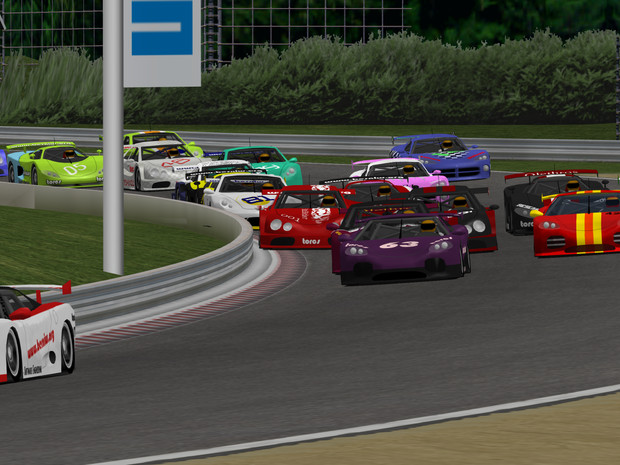
\includegraphics[height=70mm]{images/torcs.jpg}\\[1cm]

%----------------------------------------------------------------------------------------
%       DATE SECTION
%----------------------------------------------------------------------------------------

{\large \today}\\[3mm] % Date, change the \today to a set date if you want to be precise
{\large Version \docversion}\\[1.5cm]

%----------------------------------------------------------------------------------------
%       LOGO SECTION
%----------------------------------------------------------------------------------------


\includegraphics[height=13mm]{../images/logo.png} % Include a department/university logo - this will require the graphicx package

%----------------------------------------------------------------------------------------

% \vfill % Fill the rest of the page with whitespace

\end{titlepage}

  \end{titlepage}

  
  \clearpage

  \tableofcontents
  \addcontentsline{toc}{section}{Table de matière}
  
  %\vfill
  %\begin{center}
  %  
\includegraphics[height=90mm]{images/torcs.png} 
  %\end{center}

  \clearpage
  
  \renewcommand{\labelitemi}{$\bullet$}
  \renewcommand{\labelitemii}{$\circ$}
  \renewcommand{\labelitemiii}{$\diamond$}
  \renewcommand{\labelitemiv}{$\ast$}
  
  \section{Rappel des objectifs}


 
 
 \section{Choix d’implémentation}
  Décrire les principaux choix d’implémentation et les justifier.

  
  
  
  \section{Architecture du logiciel}

  
  
  
  \section{Description du code}
    \subsection{Eléments utilisés}
    Décrire rapidement les librairies et fonctions/objets utilisées.
    \subsection{Eléments produits}
    Décrire les librairies et fonctions implémentées.
    \subsection{Paramètres d’implémentation}
    Liste des paramètres de programmation (constantes, tailles maximales, etc.) 
    importants utilisés à la compilation.

\addcontentsline{toc}{section}{Références}
\bibliographystyle{../dependance/apalike}
\bibliography{../dependance/biblio}

\end{document}



